

{\large Slide 05. Planos Cristalinos e densidade planar}

\section{Planos cristalinos}
\noindent

Planos de átomos ou íons influenciam as propriedades e o comportamento dos materiais.

Os três índices não são separados por vírgulas e ficam entre parênteses.$\rightarrow$ (h k l)

Em cristais cúbicos, alguns planos constituem uma família de planos. \\ Ex: (100) (010) (001) etc $\rightarrow$ { h k l } Família de planos

No sistema hc os planos são designados por 4 índices (h k i l), que se referem a quatro eixos coordenados: 3 eixos na base do hexágono (120o entre si) e 1 eixo na vertical.


\section{Determinação do Índice de Müller - planos}


Os índices correspondem ao inverso das distâncias das interseções do plano com os eixos à origem.

São considerados os parâmetros de rede (a, b , c) como unidade para definição dos índices de Miller.

{\large CONSULTAR SLIDE PARA EXEMPLOS DE PLANOS CRISTALINOS}


\section{PLANOS CRISTALINOS vsCaracterização de estruturas}


\textbf{DIFRAÇÃO DE RAIOS-X} Técnica de caracterização estrutural de estruturas cristalinas. O bombardeamento de amostras com feixes de elétrons, gera emissão característica dos elementos constituintes.

A avaliação da estrutura cristalina pode ser feita por difratogramas produzidos por ondas que interagem com os átomos e que possuem comprimentos de onda com ordem de grandeza das distâncias interatômicas.

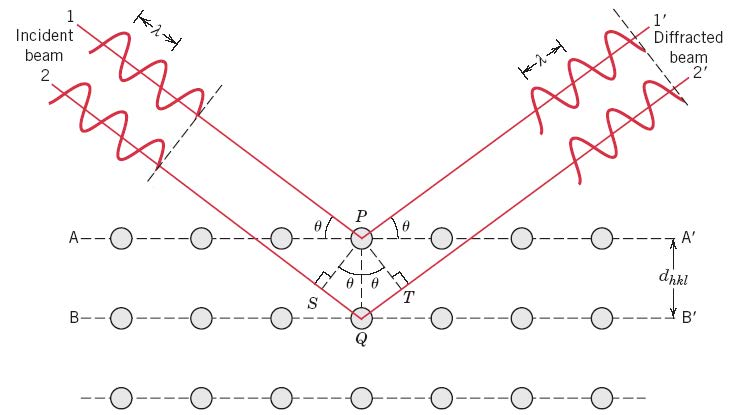
\includegraphics[scale=0.4,trim={0 0 0 0}]{figures/difracao}

Como funciona:

\begin{itemize}
	\item Incidência de feixe de raios-X com ângulo de incidência $\theta$sobre planos cristalinos com distância interplanar d.
	\item Emissão característica dos elementos constituintes.
\end{itemize}

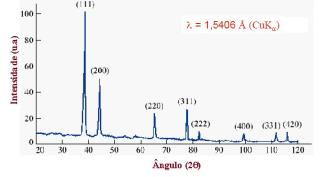
\includegraphics[scale=0.4,trim={0 0 0 0}]{figures/difratograma}

A avaliação da estrutura cristalina pode ser feita por difratogramas. Um feixe de raios-X é direcionado ao material cristalino e difratado pelos planos dos átomos ou íons com comprimentos de onda na ordem de grandeza das distâncias interatômicas.

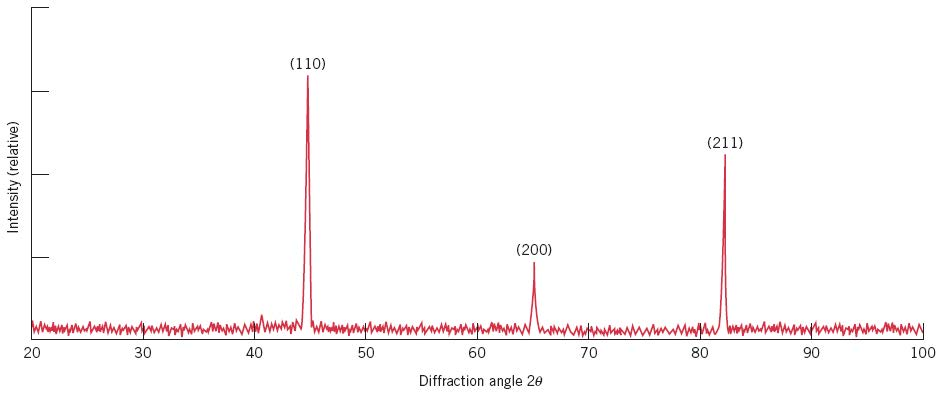
\includegraphics[scale=0.4,trim={0 0 0 0}]{figures/difraFe}

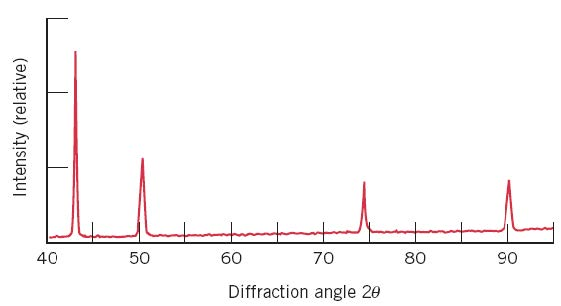
\includegraphics[scale=0.4,trim={0 0 0 0}]{figures/difraCu}

A mistura de amostras é revelada no difratograma com a superposição dos padrões individuais. Ex: Quartzo e NaCl (ver difratogramas do slide 05)


\textbf{Densidade planar}

$D_{p}$= átomos centrados sobre o plano / área do plano